\section{Interim Empirical Results}\label{sec:results}

\subsection{Predictive performance on validation and test seasons}\label{sec:results-prediction}
Table~\ref{tab:model-metrics} reports the complete validation and test comparison after temperature calibration. The uniform benchmark has test log loss 2.51622, while the market attains 2.03209. Fundamental models lie between these references: fundamental logit attains 2.24708 and fundamental LightGBM 2.24613. Their top-one strike rates are 22.85\% and 23.43\%, respectively, compared with 11.95\% for uniform and 28.65\% for market. This answers RQ1 provisionally: historical features contain substantial predictive information, but the constructed fundamental specifications remain well behind final market prices on the untouched season.

Adding market variables closes almost all of that gap. Combined logit has validation log loss 2.00168, the lowest among the four trained candidates, and is therefore the primary trained model. Its test log loss is 2.03177, only 0.000328 below the market value, and its top-one rate is 29.35\%, 0.696 percentage points above the market/favourite rate. Combined LightGBM performs slightly worse at 2.04694. The validation result also warns against overstatement: calibrated market log loss is 1.98864, better than every trained candidate, including combined logit. Thus the main finding is approximate market equivalence on test, not a consistent forecasting advantage.

\begin{table}[htbp]
\centering
\caption{Calibrated probability-model performance}\label{tab:model-metrics}
\small
\setlength{\tabcolsep}{3.5pt}
\begin{tabular}{L{3.8cm} R{1.85cm} R{1.45cm} R{1.5cm} R{1.5cm} R{1.4cm} R{1.4cm}}
\toprule
\textbf{Model} & \textbf{Validation LL} & \textbf{Test LL} & \textbf{Test Brier} & \textbf{Test top-one} & \textbf{Test ECE} & \textbf{Test AUC} \\
\midrule
Uniform & 2.49199 & 2.51622 & 0.91845 & 11.95\% & 0.00000 & 0.53248 \\
Market & \textbf{1.98864} & 2.03209 & \textbf{0.81882} & 28.65\% & 0.00573 & 0.79187 \\
Fundamental logit & 2.20062 & 2.24708 & 0.86938 & 22.85\% & 0.00672 & 0.72515 \\
Fundamental LightGBM & 2.21361 & 2.24613 & 0.86923 & 23.43\% & \textbf{0.00325} & 0.72504 \\
Combined logit & \underline{2.00168} & \textbf{2.03177} & 0.81946 & \textbf{29.35\%} & 0.00574 & \textbf{0.79198} \\
Combined LightGBM & 2.01057 & 2.04694 & 0.82213 & 28.54\% & 0.00663 & 0.78802 \\
\bottomrule
\end{tabular}
\source{Bold test entries indicate the best numerical value; the underlined validation entry identifies the primary trained candidate. Market is a benchmark, not a trained candidate. Lower LL, Brier, and ECE are better; higher top-one and AUC are better.}
\end{table}

\begin{figure}[htbp]
\centering
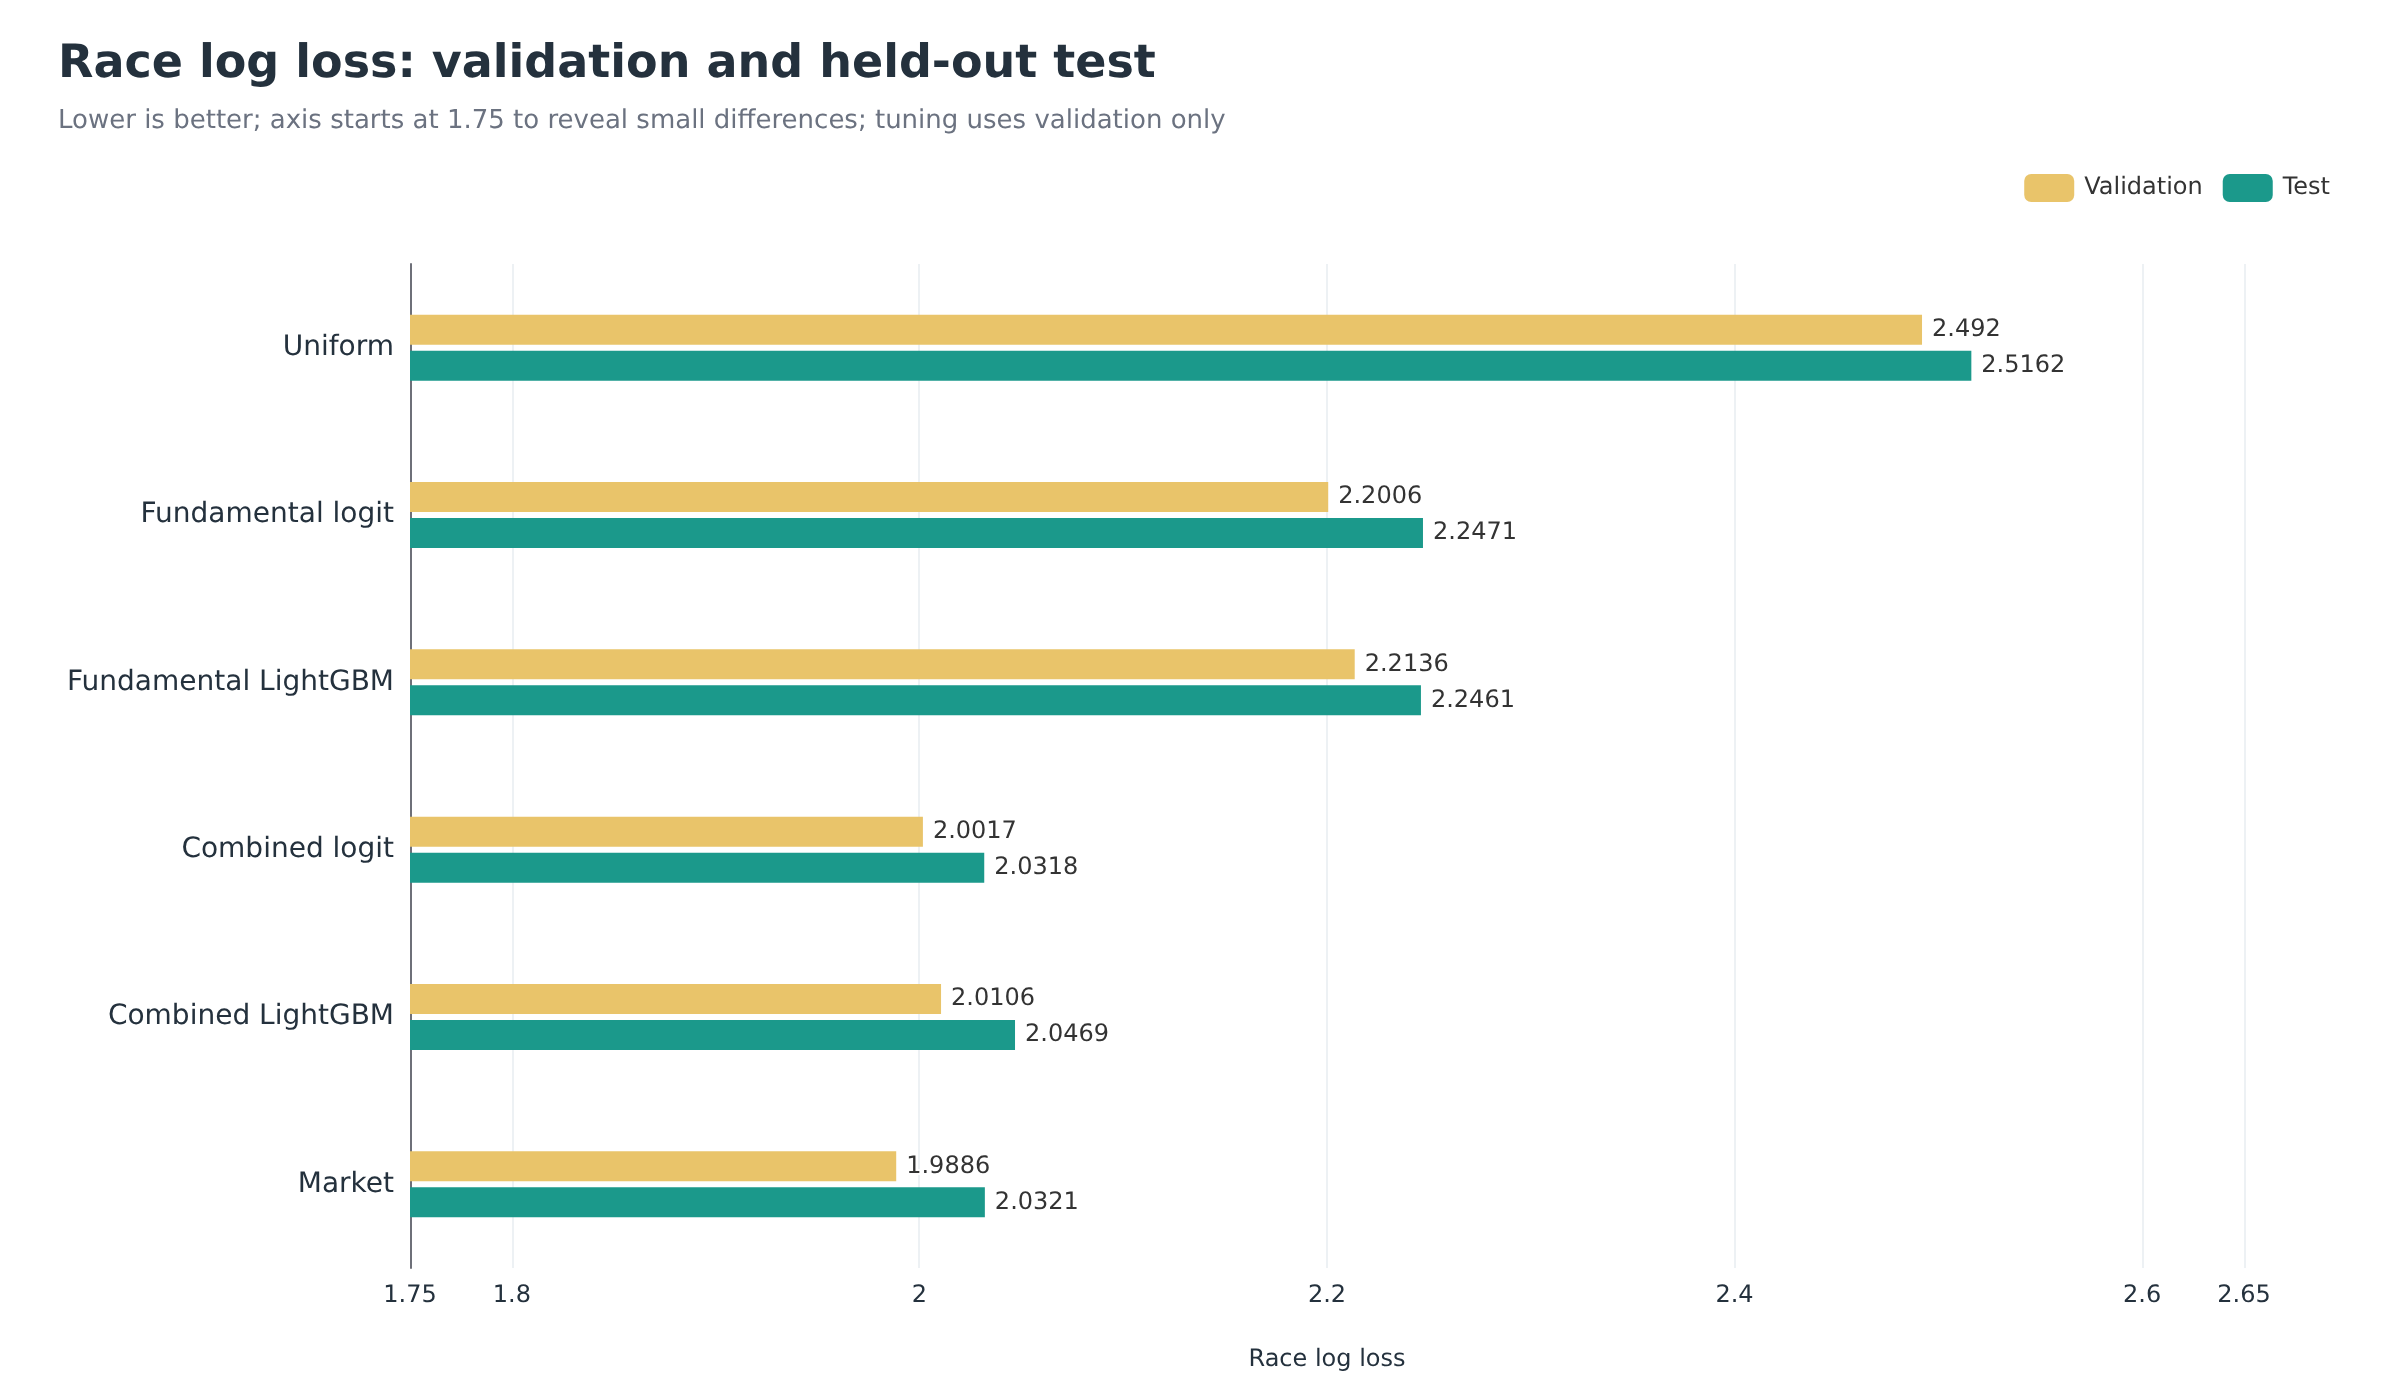
\includegraphics[width=0.97\textwidth]{model_comparison.png}
\caption{Validation and test race log loss. The horizontal axis is truncated to make small differences visible; numerical labels provide the actual scores.}\label{fig:model-comparison}
\end{figure}

Paired meeting-bootstrap intervals reinforce the cautious interpretation. For combined logit minus market, the test log-loss difference is $-0.000328$ with 95\% interval $[-0.008867,0.008288]$. The Brier difference is $+0.000650$ with interval $[-0.002300,0.003498]$, and the top-one difference is $+0.696$ percentage points with interval $[-0.692,2.100]$ points. All three intervals include zero. Combined LightGBM's log-loss difference is $+0.01484$ with interval $[0.00098,0.02900]$, indicating a small disadvantage relative to the market under this resampling analysis. Fundamental-model disadvantages are much larger and their intervals are clearly above zero for log loss.

\begin{table}[htbp]
\centering
\caption{Paired test differences: primary combined logit minus market}\label{tab:paired-differences}
\small
\begin{tabular}{L{3.4cm} R{2.5cm} R{3.5cm} L{3.9cm}}
\toprule
\textbf{Metric} & \textbf{Difference} & \textbf{95\% meeting-bootstrap interval} & \textbf{Interpretation} \\
\midrule
Race log loss & $-0.000328$ & $[-0.008867,\ 0.008288]$ & No resolved difference; negative would favour the model. \\
Multiclass Brier loss & $+0.000650$ & $[-0.002300,\ 0.003498]$ & No resolved difference; positive would favour the market. \\
Top-one strike rate & $+0.696$ pp & $[-0.692,\ 2.100]$ pp & No resolved difference; positive would favour the model. \\
\bottomrule
\end{tabular}
\source{5,000 paired meeting-cluster resamples; pp denotes percentage points.}
\end{table}

\subsection{Calibration and reliability}\label{sec:results-calibration}
Global ECE values are small in absolute terms, ranging from 0.00325 for fundamental LightGBM to 0.00672 for fundamental logit among the non-degenerate models. Figure~\ref{fig:reliability} shows why these summaries should still be accompanied by bin-level inspection. Market, combined-logit, and fundamental-LightGBM probabilities broadly follow the diagonal, but deviations vary across the probability range. In the highest market decile, for example, mean predicted probability is 30.08\% and observed frequency is 28.44\%; in the preceding decile, prediction is 15.70\% and observation 16.73\%. A single global temperature cannot remove all such local differences.

The reliability curves also show that the fundamental model is not uninformative. Its probabilities span a useful range and track observed frequencies approximately, despite weaker log loss and discrimination than the market. This pattern is consistent with information that is genuinely predictive but already largely incorporated into prices. The near-unit combined-logit temperature (1.00260) suggests that its validation likelihood required negligible global sharpening or softening. By contrast, the market temperature of 0.91977 sharpens normalized market probabilities. These are global parameters fitted on one validation season, so their stability across alternative periods remains a final-stage question.

\begin{figure}[htbp]
\centering
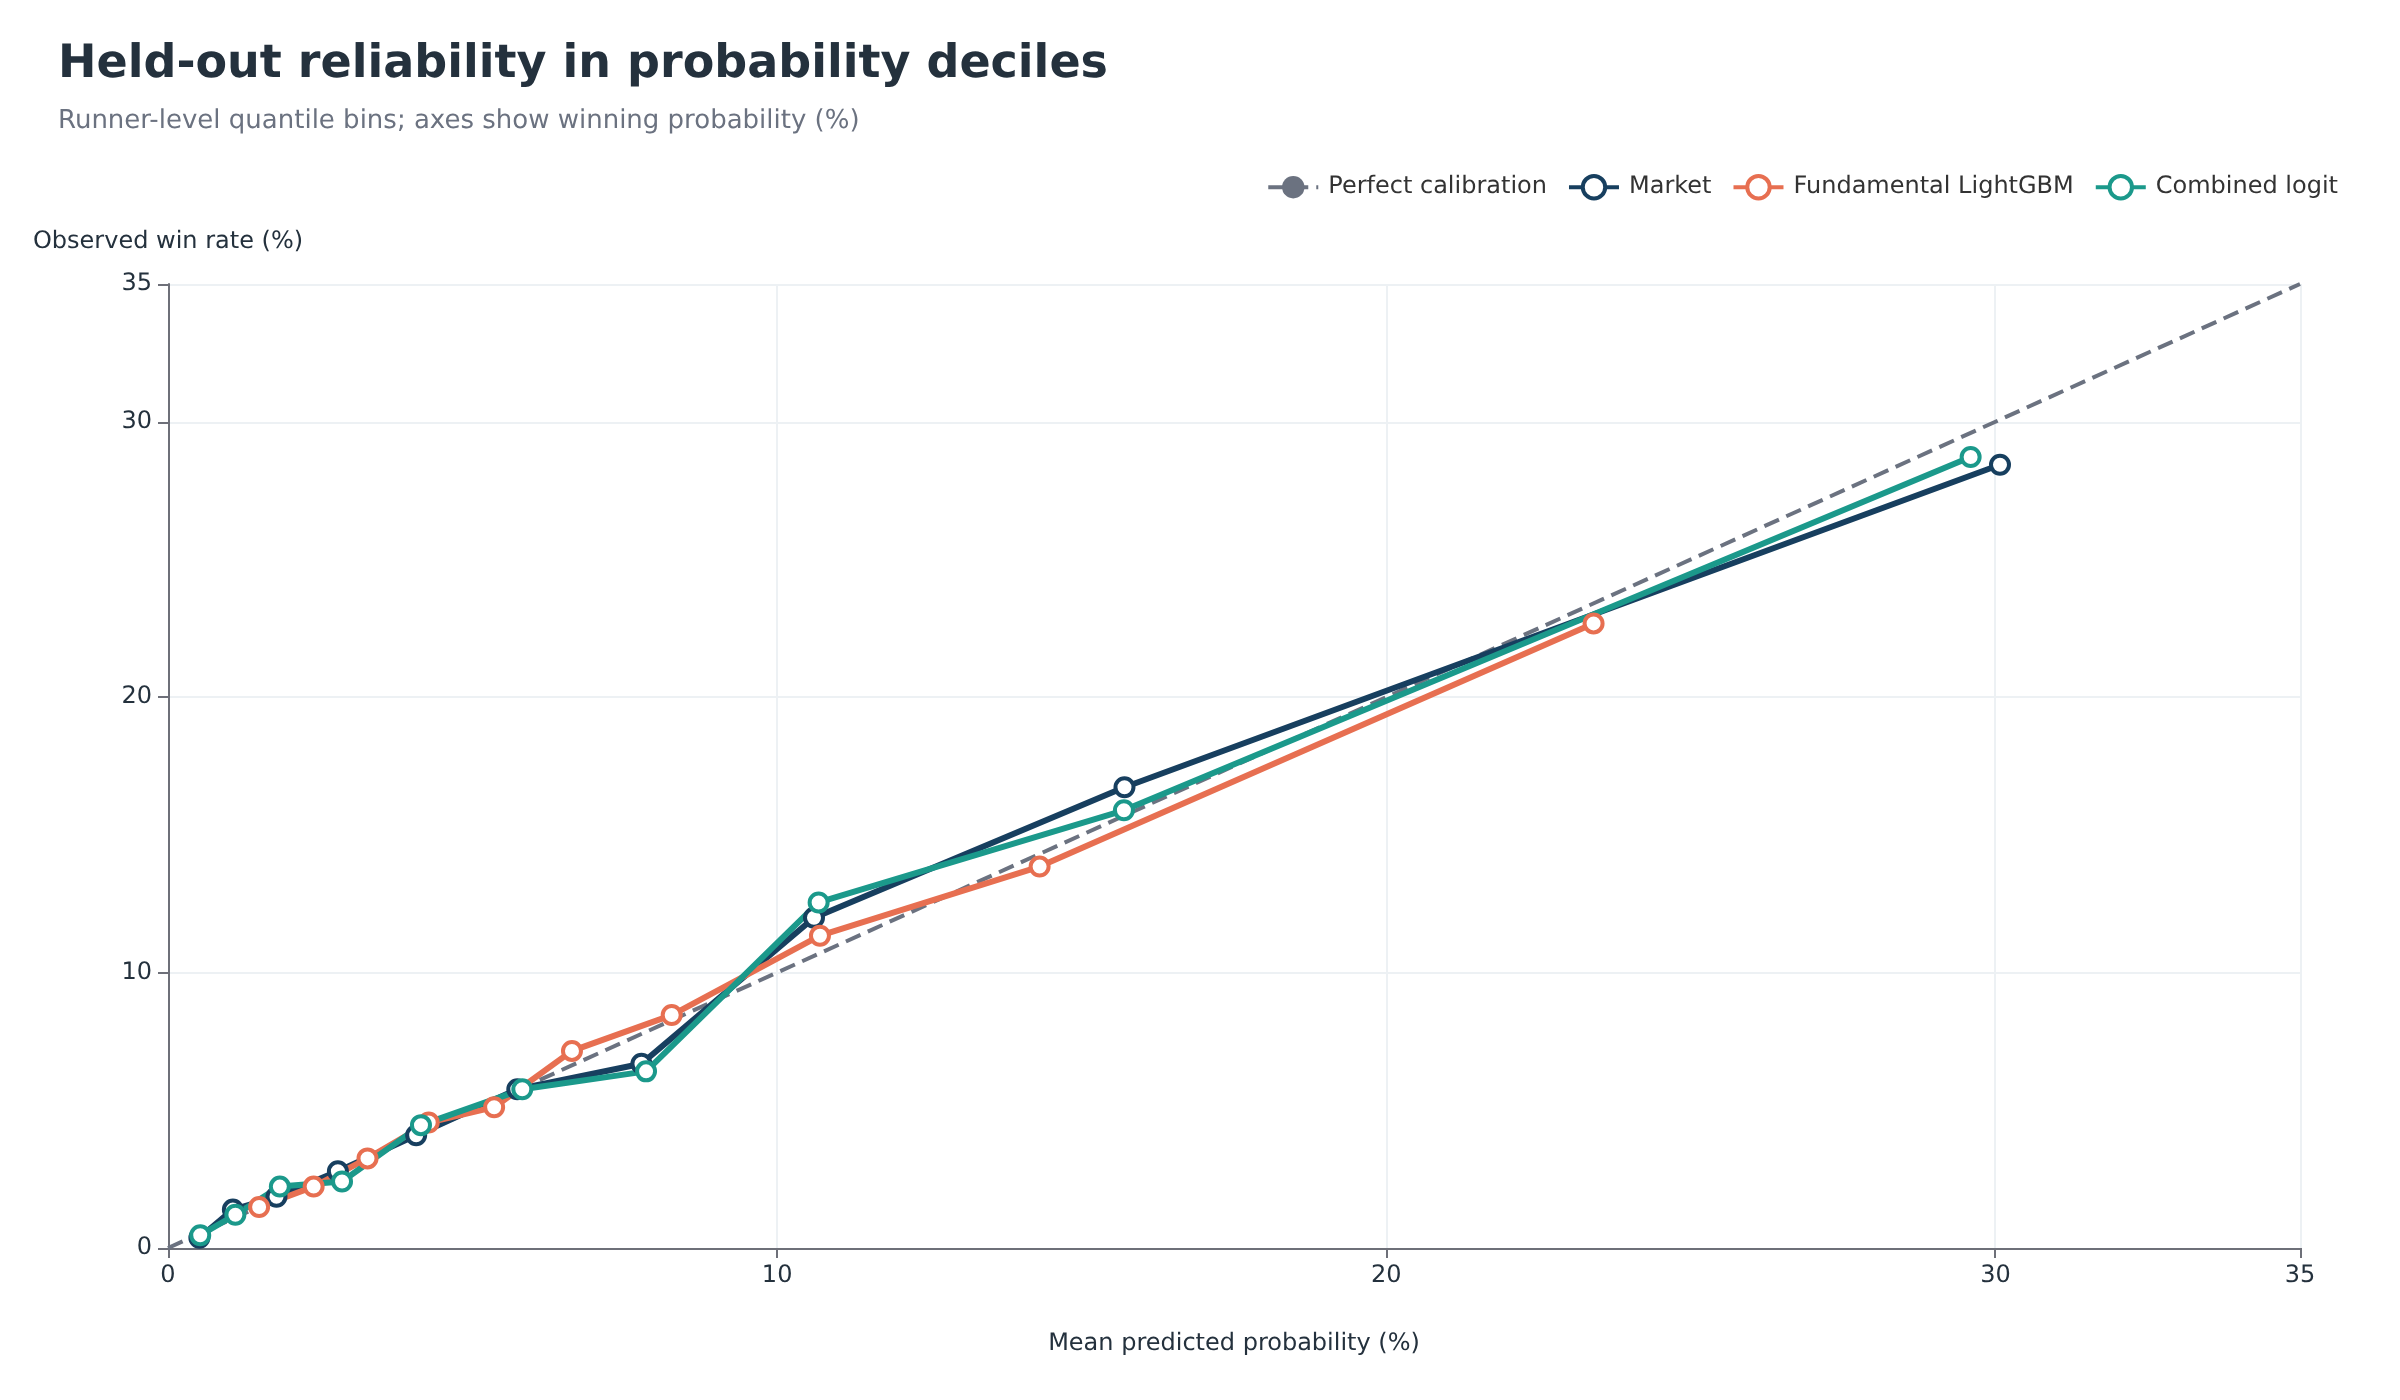
\includegraphics[width=0.96\textwidth]{reliability.png}
\caption{Held-out reliability curves using ten runner-level quantile bins per model. The dashed line denotes perfect calibration.}\label{fig:reliability}
\end{figure}

\subsection{Feature importance and model behaviour}\label{sec:results-importance}
Figure~\ref{fig:importance} displays LightGBM gain importance. In the fundamental model, last-three finishing form contributes 24.27\% of total gain, most recent finish 13.94\%, jockey mean finish 9.64\%, jockey place rate 5.86\%, and normalized draw 3.52\%. The prominence of recent form is consistent with the modeling rationale, but the values are not causal effects. Correlated variables can share or substitute for one another across trees, and gain importance measures use within the fitted ensemble rather than independent information content.

The combined model is dominated by final market variables: log WIN odds contribute 42.32\% and log normalized market probability 36.47\%, together 78.79\% of total gain. Relative carried weight is a distant third at 1.43\%. This concentration explains why adding fundamental variables produces only a small change relative to the market benchmark. It also cautions against interpreting the two market columns separately because they are deterministically related within a race. Future ablation and two-stage residual modeling will be more informative than adding further correlated transformations of the same final price.

\begin{figure}[htbp]
\centering
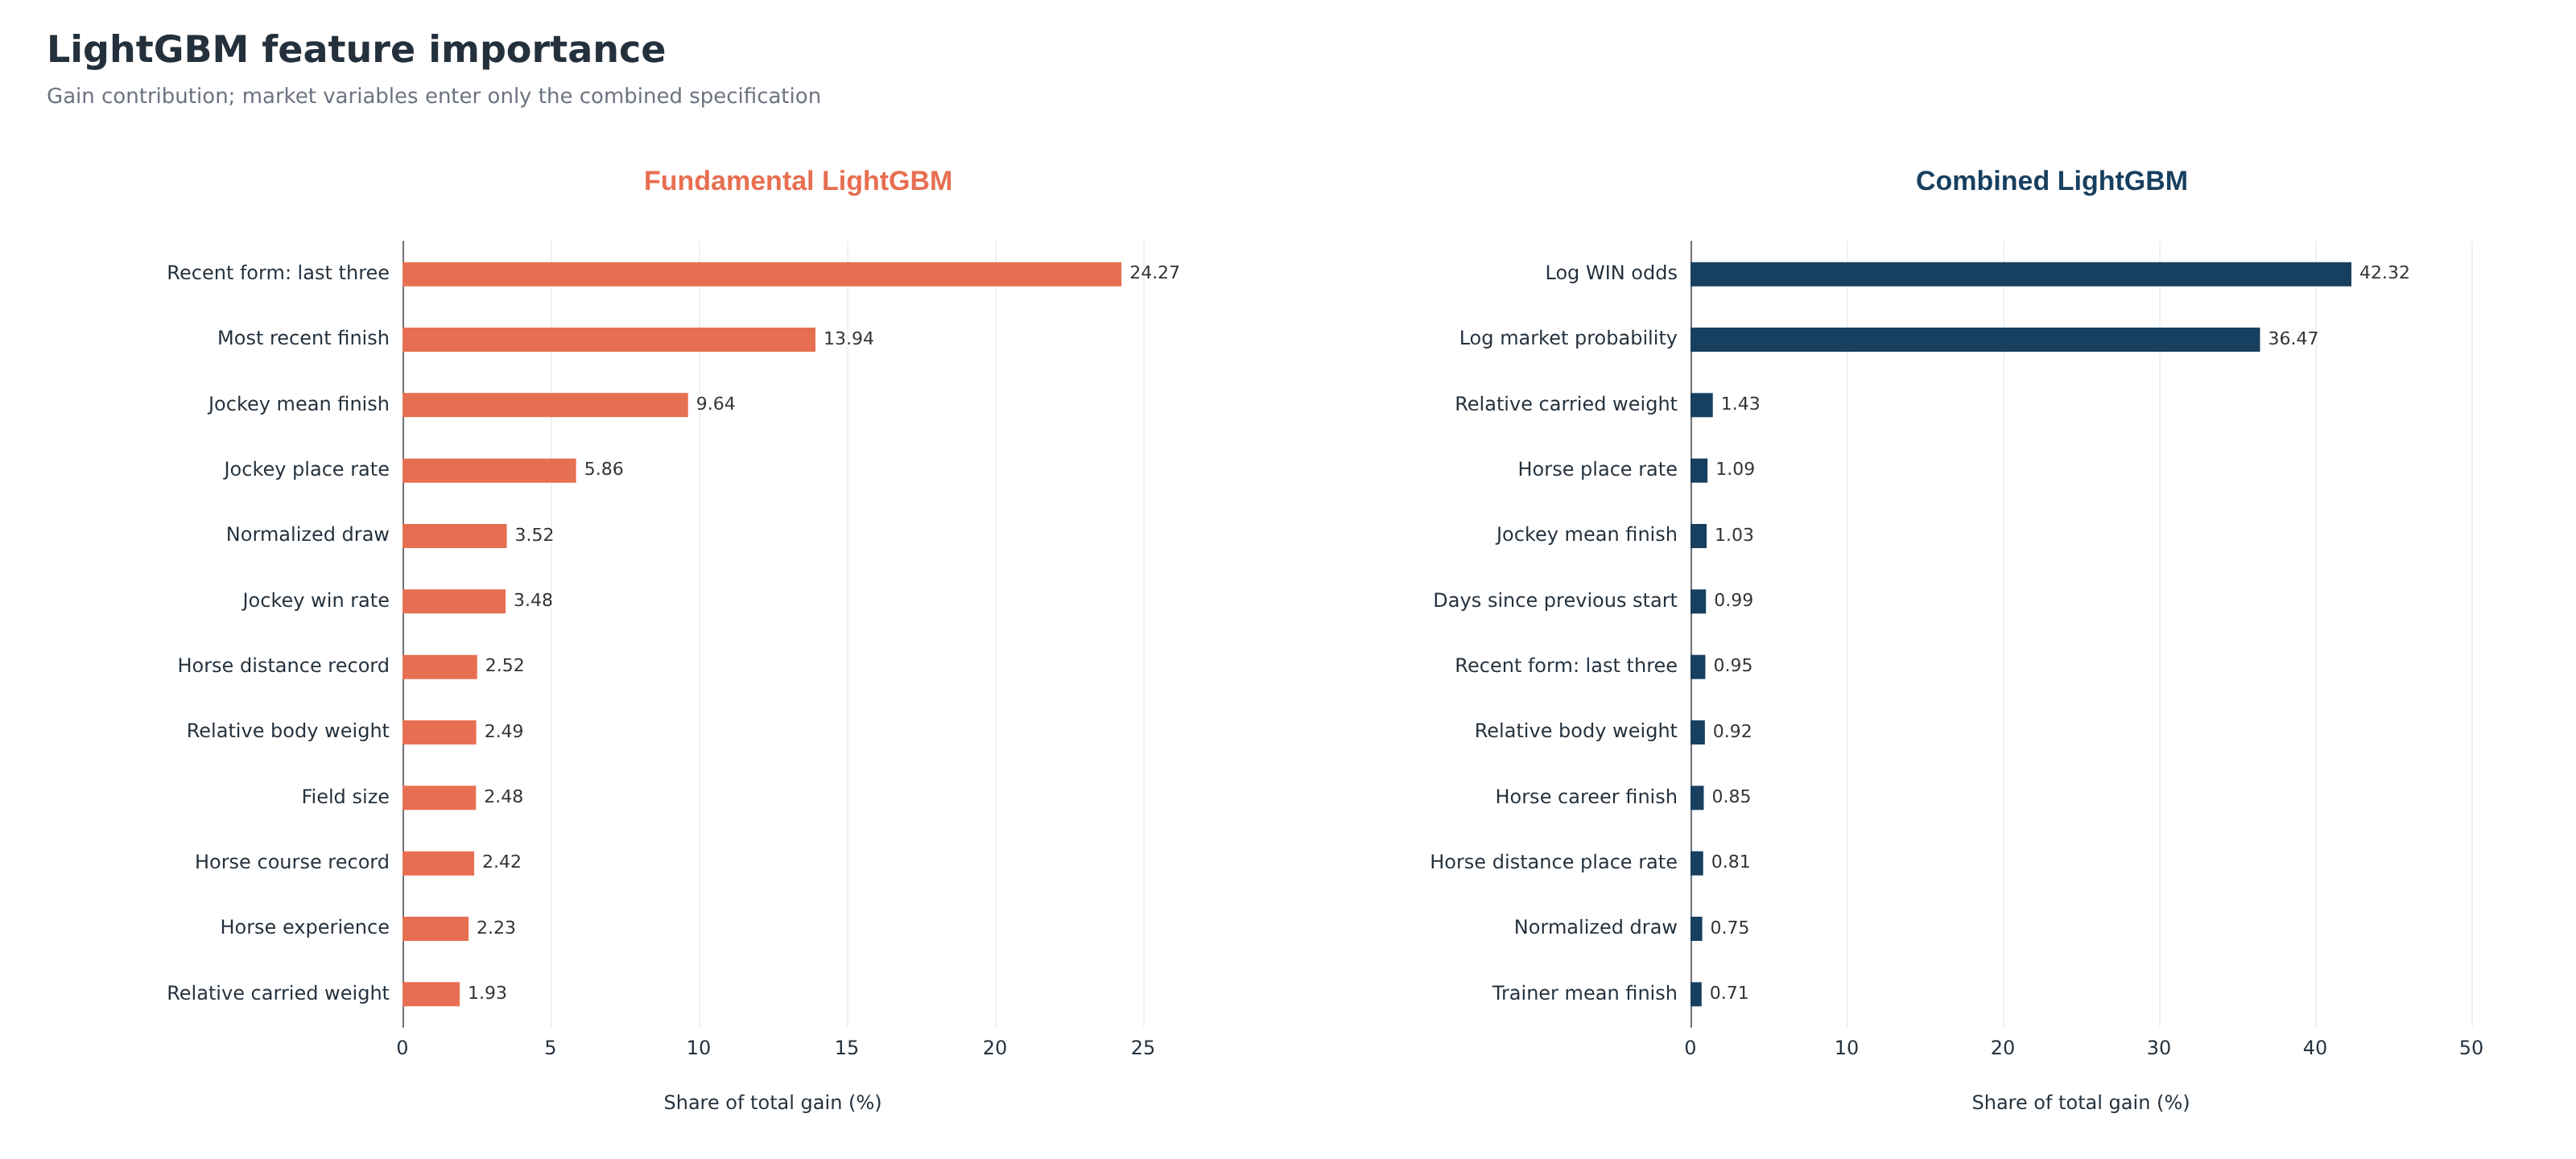
\includegraphics[width=0.99\textwidth]{feature_importance.png}
\caption{LightGBM gain importance for the twelve largest contributors in each specification. Percentages sum over all ensemble features, not only the displayed subset.}\label{fig:importance}
\end{figure}

\subsection{Odds-band calibration and unconditional returns}\label{sec:results-odds}
Before examining model-selected bets, it is useful to ask whether simple price bands already show strong market patterns. Figure~\ref{fig:odds-bands} compares mean normalized market probability with observed win frequency and reports ROI from betting HK\$10 on every runner in each test-season odds band. The two probability series are generally close in low and middle bands. At odds above 100, however, only one of 796 runners wins: the observed rate is 0.126\%, compared with a mean normalized market probability of 0.593\%, and the band ROI is $-80.1\%$. One sparse bin cannot establish a stable structural bias, but it illustrates the danger of indiscriminate longshot betting.

Every displayed odds band has a negative unconditional ROI in the test season. The losses range from $-12.1\%$ for displayed odds 50.1--100 to $-80.1\%$ above 100; favourites at odds 1.0--2.0 lose 17.7\%, and the 2.1--4.0 band loses 16.9\%. These outcomes do not reproduce a simple claim that favourites always offer favourable value, nor do they prove a universal favourite--longshot law. They are one-season empirical frequencies subject to sampling variation and official-dividend rounding. They do, however, establish a demanding baseline for any claim that a model has found exploitable prices.

\begin{figure}[htbp]
\centering
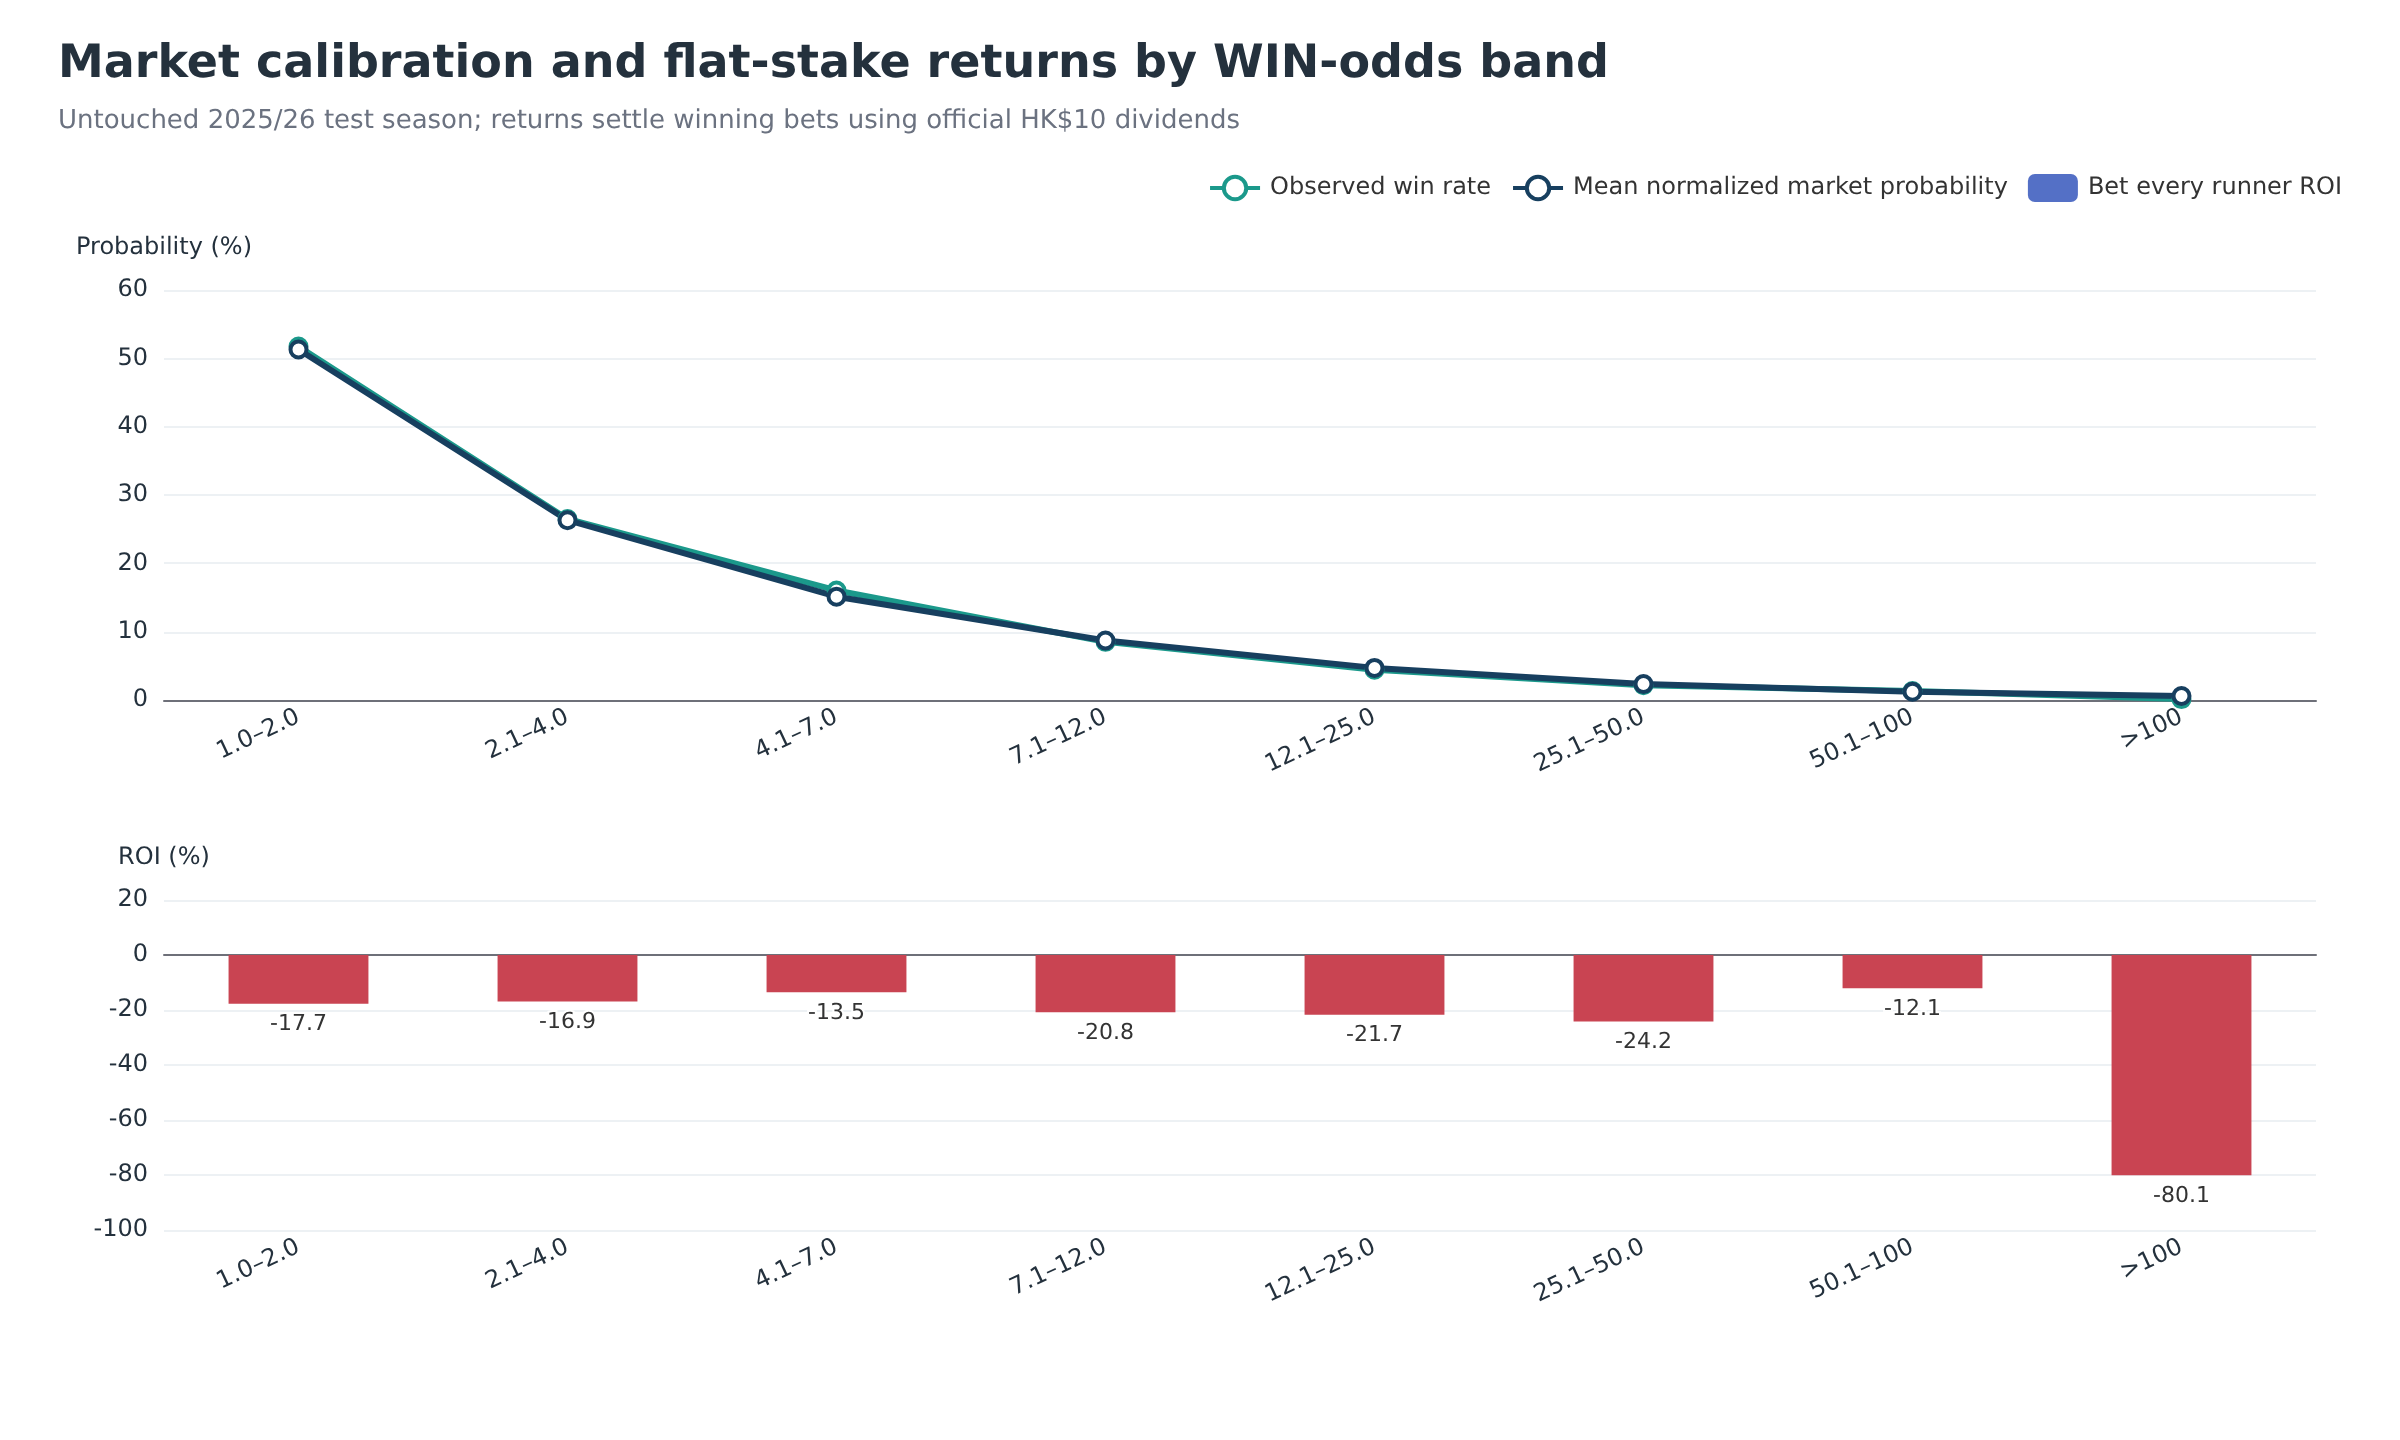
\includegraphics[width=0.98\textwidth]{odds_bands.png}
\caption{Test-season market calibration and unconditional flat-stake returns by displayed WIN-odds band. The upper panel uses all runners; the lower panel bets HK\$10 on every runner and settles from official dividends.}\label{fig:odds-bands}
\end{figure}

\subsection{Prespecified betting evaluation}\label{sec:results-betting}
The primary combined-logit value rule qualifies in 127 of 862 test races, spread across 68 meetings. It stakes HK\$1,270 and returns a net profit of HK\$91, corresponding to ROI 7.17\%. The strike rate is 14.17\%, mean displayed odds are 9.51, and maximum drawdown is HK\$287. Although the point estimate is positive, the meeting-cluster 95\% ROI interval is $[-49.56\%,77.19\%]$. Only 18 of the 127 selections win, so a small number of payouts materially affects the result. The appropriate conclusion is that the interim data are compatible with both meaningful gains and substantial losses, not that a profitable system has been demonstrated.

Alternative strategies are generally negative. Betting the primary model's top-probability runner in every race produces 29.35\% winners but loses HK\$1,399 on HK\$8,620 staked (ROI $-16.23\%$). This is less negative than the favourite-every-race ROI of $-19.94\%$, but both lose money. Combined-LightGBM value betting loses 2.12\% over 481 bets; fundamental-logit and fundamental-LightGBM value rules lose 31.85\% and 14.32\%, respectively. Betting every runner loses HK\$25,342.50 on HK\$107,600 staked (ROI $-23.55\%$). The contrast between top-one accuracy and negative return directly supports the project's separation of probability quality and economic value.

\begin{table}[htbp]
\centering
\caption{Selected test-season betting outcomes at HK\$10 flat stakes}\label{tab:betting-main}
\scriptsize
\setlength{\tabcolsep}{2.5pt}
\begin{tabular}{L{3.1cm} R{1.0cm} R{1.5cm} R{1.9cm} R{1.35cm} R{1.2cm} R{1.25cm} L{3.0cm}}
\toprule
\textbf{Strategy} & \textbf{Bets} & \textbf{Stake HK\$} & \textbf{Profit HK\$} & \textbf{ROI} & \textbf{Strike rate} & \textbf{Max DD HK\$} & \textbf{95\% ROI interval} \\
\midrule
Combined logit value & 127 & \num{1270} & $+91.00$ & $+7.17\%$ & 14.17\% & 287.00 & $[-49.56\%,77.19\%]$ \\
Combined logit top pick & 862 & \num{8620} & $-\num{1399.00}$ & $-16.23\%$ & 29.35\% & \num{1525.00} & $[-25.95\%,-7.09\%]$ \\
Combined LightGBM value & 481 & \num{4810} & $-102.00$ & $-2.12\%$ & 12.89\% & 529.50 & $[-30.61\%,28.67\%]$ \\
Fundamental logit value & 833 & \num{8330} & $-\num{2653.00}$ & $-31.85\%$ & 5.52\% & \num{3035.50} & $[-53.27\%,-9.16\%]$ \\
Fundamental LightGBM value & 840 & \num{8400} & $-\num{1203.00}$ & $-14.32\%$ & 6.19\% & \num{2755.00} & $[-39.16\%,12.25\%]$ \\
Favourite every race & 862 & \num{8620} & $-\num{1718.50}$ & $-19.94\%$ & 28.65\% & \num{1718.50} & $[-29.51\%,-10.58\%]$ \\
Every runner & \num{10760} & \num{107600} & $-\num{25342.50}$ & $-23.55\%$ & 8.01\% & --- & --- \\
\bottomrule
\end{tabular}
\source{Official WIN dividends settle winners. Intervals use 3,000 meeting-cluster resamples. The every-runner baseline has no selection bootstrap or drawdown entry.}
\end{table}

Figure~\ref{fig:cumulative-profit} shows the time path behind the summary statistics. The primary value balance rises through some parts of the season but also experiences extended flat and declining intervals; its final HK\$91 profit is small relative to the path's fluctuations and to total stakes. The favourite strategy declines much more persistently and ends at HK\$-1,718.50. A cumulative graph is useful for identifying sequence and drawdown, but it does not add independent evidence beyond the same 862 races. It should therefore be read together with, rather than instead of, the clustered intervals and sensitivity analysis.

\begin{figure}[htbp]
\centering
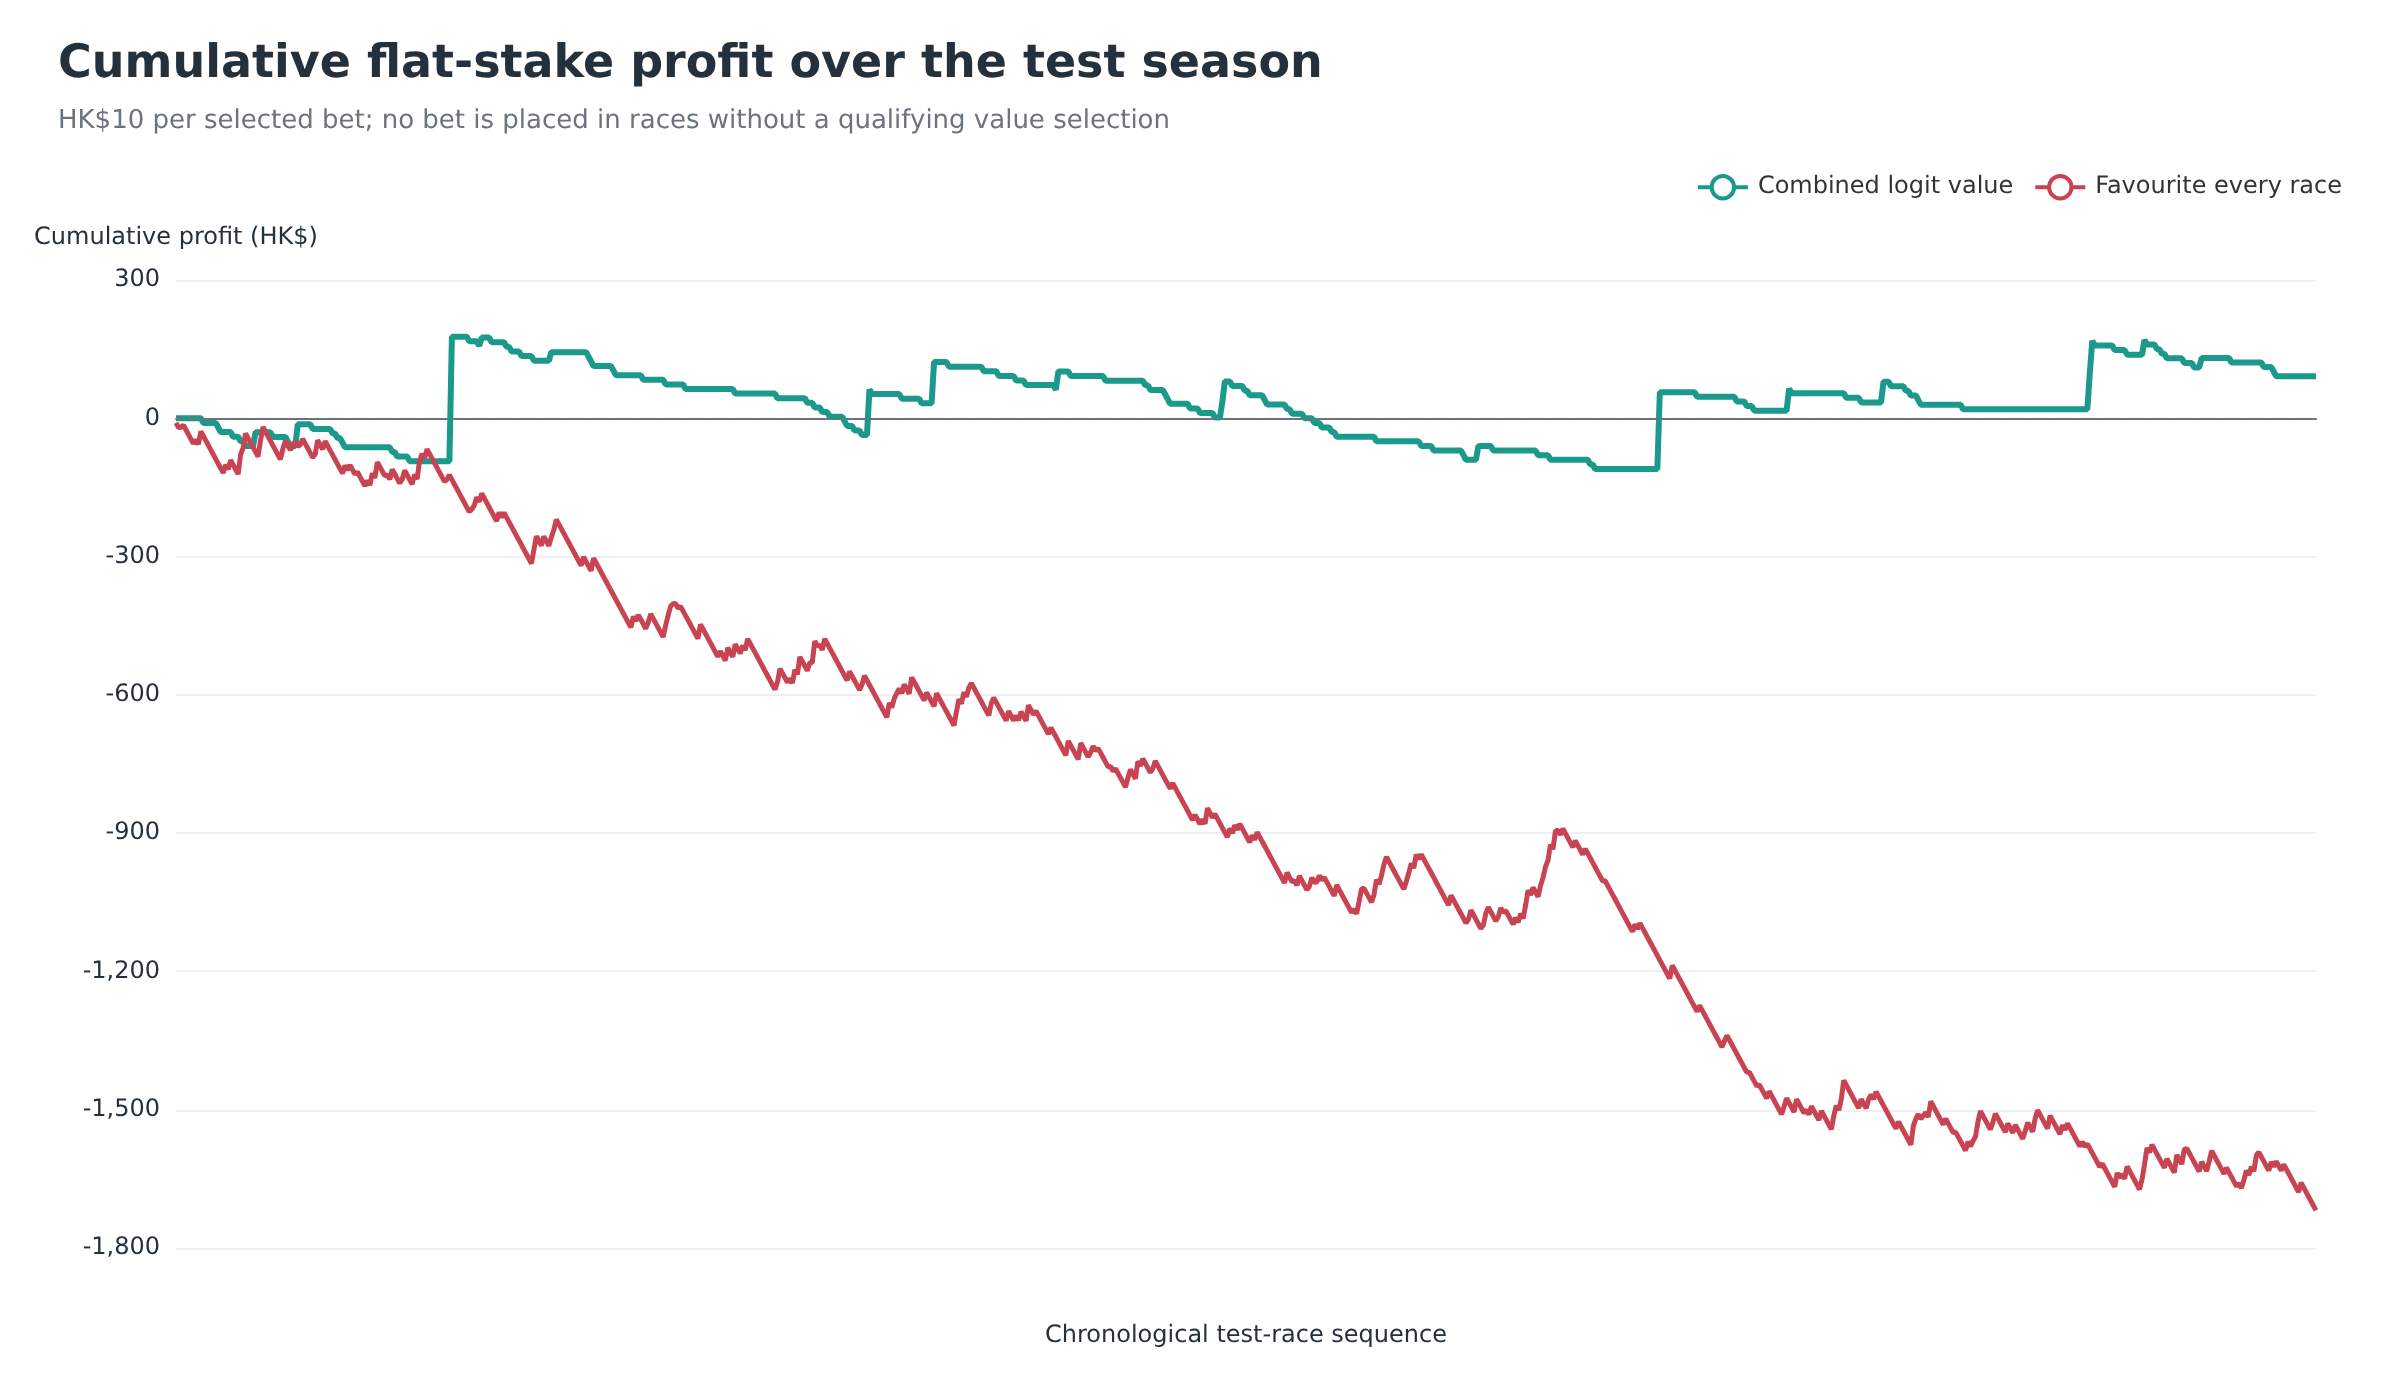
\includegraphics[width=0.97\textwidth]{cumulative_profit.png}
\caption{Cumulative test-season profit for the primary value rule and favourite-every-race baseline. Flat portions of the value series represent chronological races without a qualifying selection.}\label{fig:cumulative-profit}
\end{figure}

\subsection{Threshold sensitivity and robustness}\label{sec:results-sensitivity}
Figure~\ref{fig:sensitivity} varies the expected-value threshold and maximum odds for the primary model. The results are not monotone. With no edge requirement and an odds cap of 30, ROI is $-8.7\%$ over 269 bets; the prespecified 5\% edge and cap of 30 produce $+7.2\%$ over 127 bets; and a 10\% edge with the same cap produces $+65.9\%$ over only 48 bets. At a 20\% threshold, just four bets qualify and all lose, giving $-100\%$ ROI. No bets qualify at 30\%. Reducing the cap to ten under the 5\% rule produces $+5.5\%$ over 93 bets, whereas a cap of 20 produces $-1.1\%$ over 117.

These variations undermine any strong claim based on the positive primary cell. The most profitable cells contain fewer observations, and small changes in threshold move both the sign and magnitude of returns. The grid is therefore reported as an exploratory robustness diagnostic, not used to select a new ``optimal'' rule on the test season. A confirmatory final-stage analysis would need to freeze any revised rule using training/validation evidence and evaluate it on new data. At present, RQ4 is answered negatively in the robust sense: one positive point estimate exists, but profitability is not stable enough to support a reliable economic conclusion.

\begin{figure}[htbp]
\centering
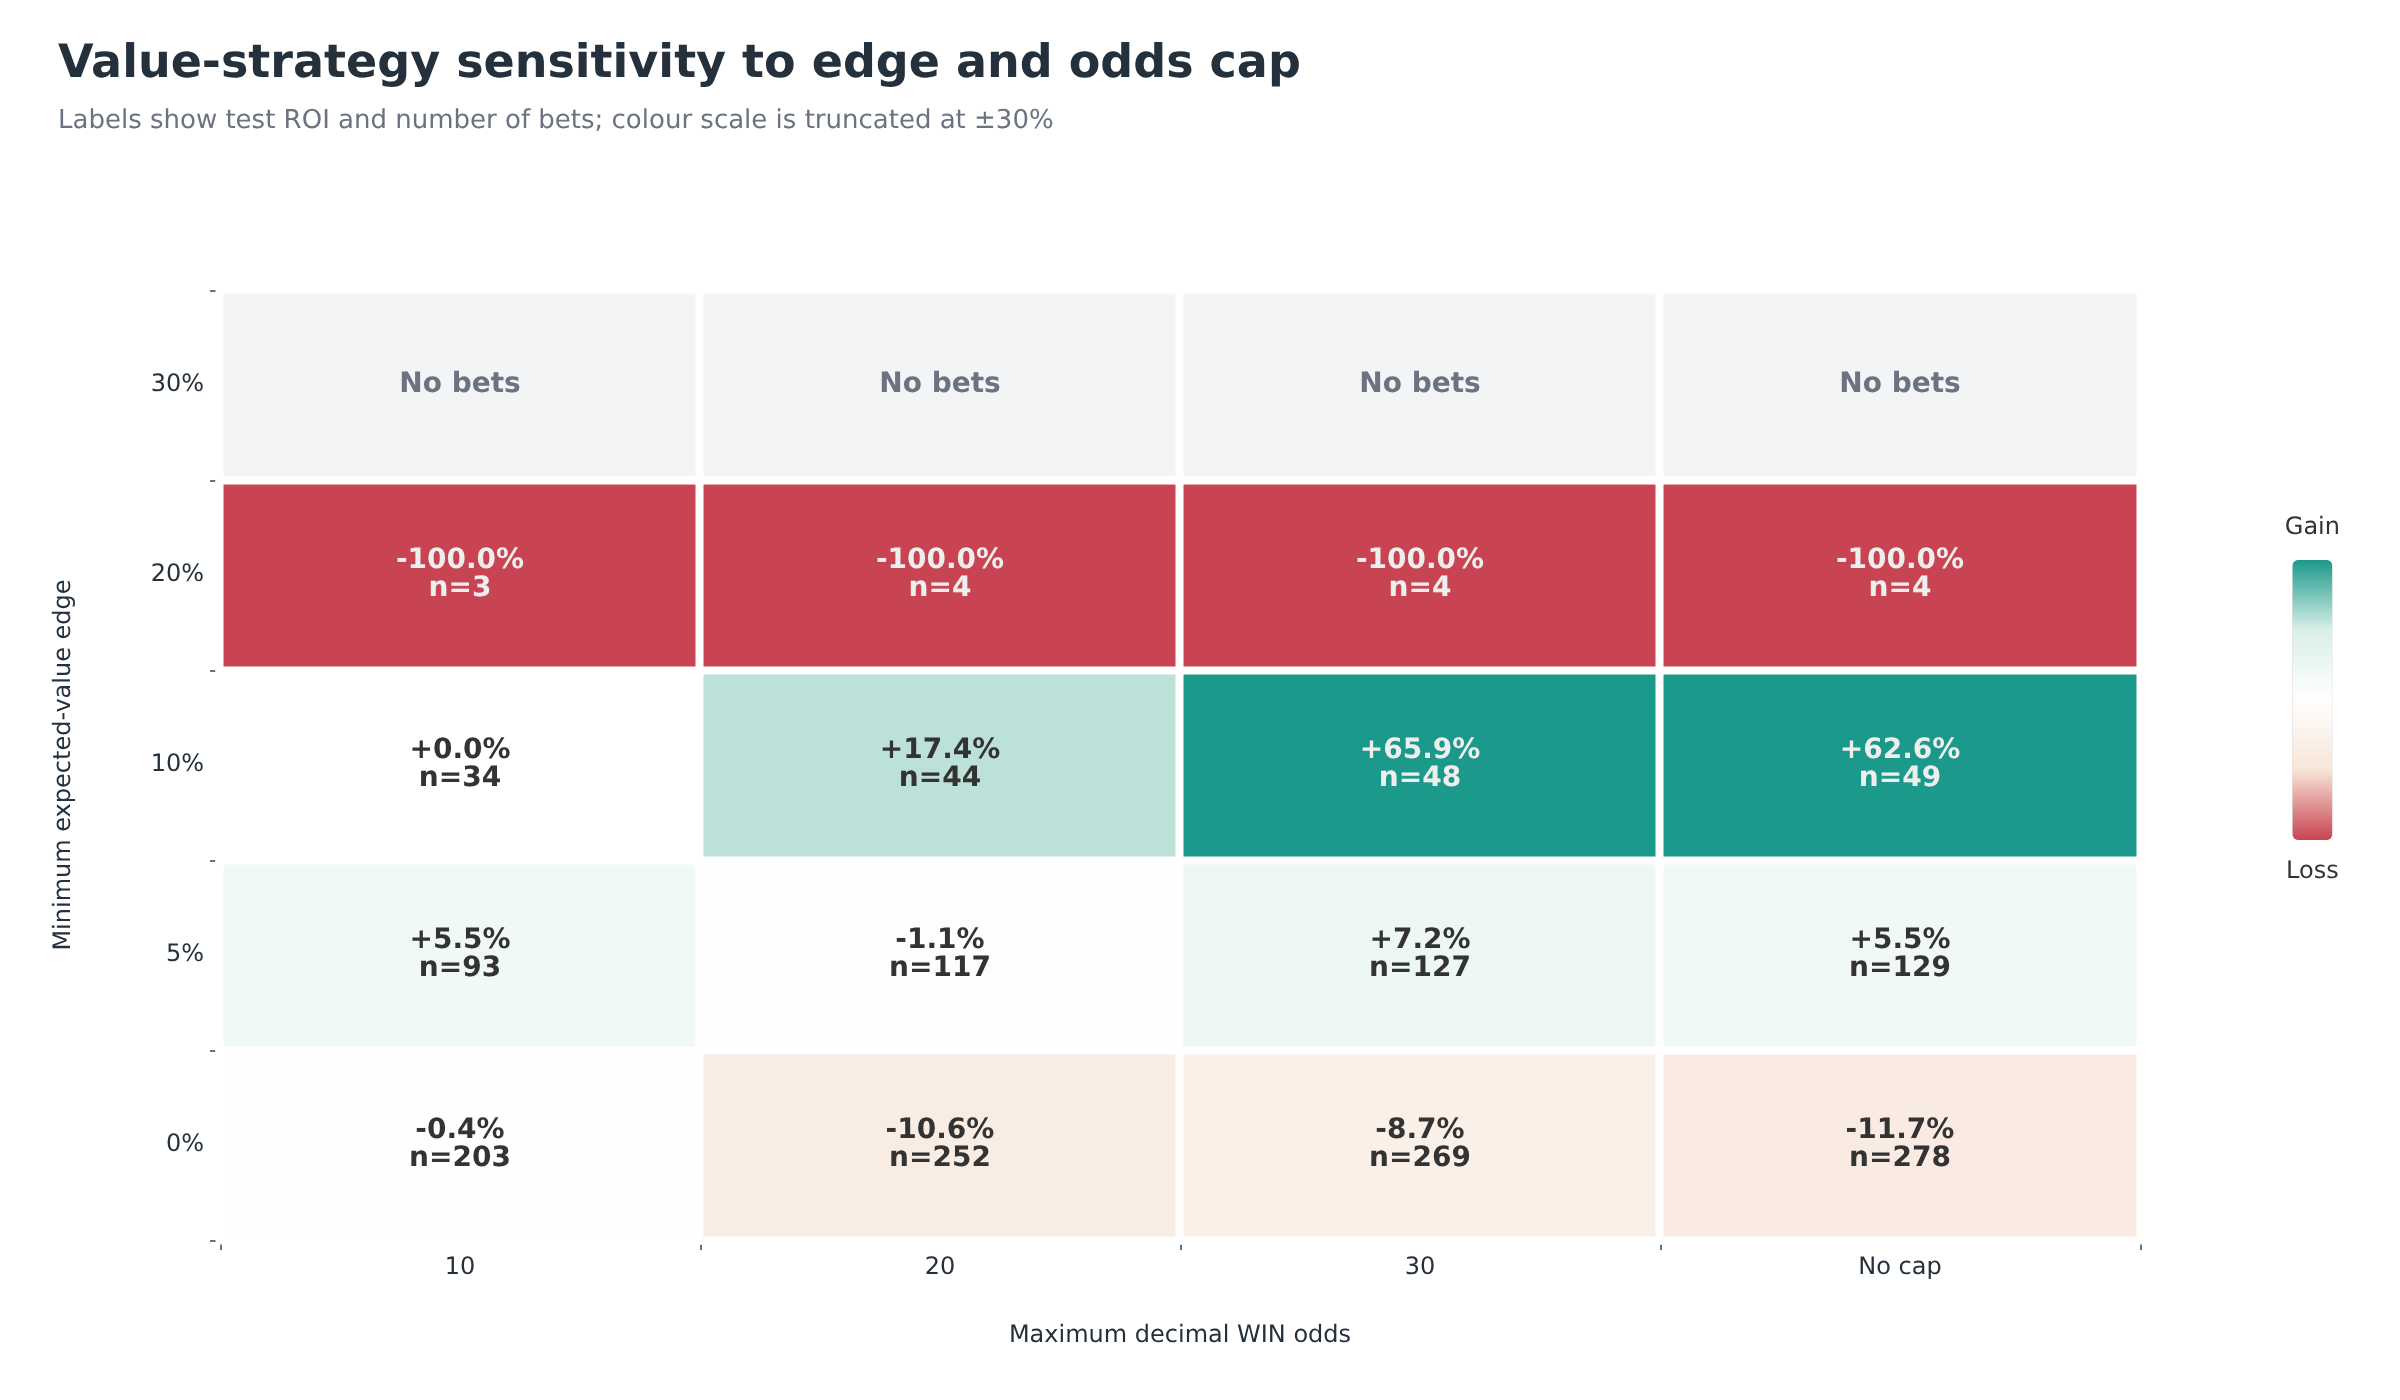
\includegraphics[width=0.97\textwidth]{betting_sensitivity.png}
\caption{Exploratory test-season sensitivity of the primary value rule. Labels show ROI and number of bets. The colour scale is truncated at $\pm30\%$ so that moderate cells remain distinguishable.}\label{fig:sensitivity}
\end{figure}
